\documentclass[11pt,a4paper]{article}

\usepackage[margin=0.8in]{geometry}
\usepackage{amsmath}
\usepackage{graphicx}
\usepackage[table]{xcolor}
\usepackage{hyperref}
\usepackage{array}
\usepackage{longtable}
\usepackage{titlesec}
\usepackage{setspace}

\hypersetup{hidelinks}
\setlength{\parskip}{0.45em}
\setlength{\parindent}{0pt}
\renewcommand{\arraystretch}{1.2}
\setlength{\extrarowheight}{2pt}

\definecolor{TitleBlue}{HTML}{153E75}
\definecolor{SoftBlue}{HTML}{EAF2FF}
\definecolor{SoftGray}{HTML}{F5F7FA}
\definecolor{RiskGreen}{HTML}{37B24D}
\definecolor{RiskDkGreen}{HTML}{2B8A3E}
\definecolor{RiskYellow}{HTML}{FEE440}
\definecolor{RiskOrange}{HTML}{FF922B}
\definecolor{RiskRed}{HTML}{F03E3E}
\definecolor{RiskDkRed}{HTML}{C92A2A}

\titleformat{\section}{\large\bfseries\color{TitleBlue}}{\thesection.}{0.5em}{}
\titleformat{\subsection}{\normalsize\bfseries\color{TitleBlue}}{\thesubsection}{0.5em}{}

\begin{document}

\begin{center}
{\LARGE\bfseries\color{TitleBlue} PHC Integrated Digital System}\\[0.3em]
{\Large Group1\_Lab910}\\[0.6em]
{\large Lab 9 \& 10 Report: Software Metrics and Risk Handling}\\[0.8em]
{\normalsize Bavadiya Yash Kiritbhai \quad Chaitanya Singh \quad Nayan Patidar}\\[0.3em]
{\normalsize IIT Jodhpur}\\[0.8em]
\fcolorbox{TitleBlue}{SoftBlue}{\parbox{0.92\linewidth}{
\textbf{Report intent.} This report tells the project story as one connected narrative: how the PHC system evolved sprint by sprint, what the repository proves today, which metrics matter, where the real risks emerged, and how those risks were already folded back into planning and backlog decisions.}}
\end{center}

\section{Project Story and Evidence Baseline}
The PHC Integrated Digital System started as a documentation-heavy academic project, but by the end of Sprint 5 it had become a working backend platform with authentication, patient records, visit lifecycle management, prescription handling, laboratory flows, billing, appointments, notifications, and admin reporting. That progression matters for this lab because the requested metrics are meaningful only if they are tied to the actual engineering story rather than to abstract estimates.

For this report, we used the current repository as the evidence baseline. The measured story comes from \texttt{README.md}, \texttt{TESTING.md}, \texttt{test\_cases.csv}, \texttt{backend/prisma/schema.prisma}, all backend route and service files, Software Requirements Specification (SRS) revisions through Version 2.2, and git history from January 15, 2026 to April 3, 2026. The resulting snapshot is:

\begin{center}
\rowcolors{2}{SoftGray}{white}
\begin{tabular}{|p{8cm}|p{4cm}|}
\hline
\rowcolor{SoftBlue}
\textbf{Repository-backed baseline} & \textbf{Measured value} \\
\hline
Production source lines of code & 2859 \\
Backend source lines of code & 2505 \\
Service-layer source lines of code & 1608 \\
Persisted domain models & 20 \\
Implemented API endpoints & 57 \\
Documented categorized test cases & 48 \\
Feature commits in the active project window & 21 \\
\hline
\end{tabular}
\end{center}

The most useful qualitative observation from this baseline is that the project is backend-heavy by design. The service layer contains most of the domain logic, which is exactly what we would expect from a system where correctness, traceability, and role safety matter more than early frontend polish.

\subsection{Late Sprint 5 Closeout Evidence}
Because Sprint 5 was the backend integration sprint, the latest repository evidence is concentrated near the end of March 2026. The sequence below is the corrected chronology used for the tracker and for this report.

\begin{center}
\rowcolors{2}{SoftGray}{white}
\begin{tabular}{|p{1.9cm}|p{2cm}|p{4.1cm}|p{6.7cm}|}
\hline
\rowcolor{SoftBlue}
\textbf{Date} & \textbf{Commit} & \textbf{Sprint 5 item} & \textbf{Meaning in the project story} \\
\hline
2026-03-25 & \texttt{9e3e7c0} & Local LDAP-backed authentication & Converted authentication from the earlier dev fallback approach into a proper local LDAP bind flow for seeded users. \\
\hline
2026-03-25 & \texttt{3fac9c2} & Full-system E2E runner & Added a repository-backed end-to-end validation path across the major backend modules. \\
\hline
2026-03-25 & \texttt{2d7e421} & Sprint 5 integration docs closeout & Synchronized API documentation and backend integration evidence near sprint closeout. \\
\hline
2026-03-25 & \texttt{9182fcc} & Availability notifications & Added doctor unavailability and in-app notification logic, reducing operational ambiguity. \\
\hline
2026-03-24 & \texttt{5ff16c2} & Admin user management & Added administrative account creation, listing, status control, and role updates. \\
\hline
2026-03-24 & \texttt{248d70a} & Usage and attendance reports & Added management-facing reporting endpoints for usage and doctor attendance summaries. \\
\hline
2026-03-24 & \texttt{b66f7f2} & PHC events module & Added event publishing and public event visibility for PHC communication. \\
\hline
2026-03-24 & \texttt{7718df7} & Patient lab report access & Added role-safe patient access to their own laboratory reports. \\
\hline
2026-03-24 & \texttt{f1ef67b} & Lab request detail endpoint & Added single-request detail retrieval with access control checks. \\
\hline
\end{tabular}
\end{center}

\section{Section I: Metrics and Their Meaning}
\subsection{Metric Scope and Evidence}
To keep the numbers defensible, we did not treat the whole repository as one undifferentiated code dump. Size-oriented metrics such as COCOMO and Halstead were computed from the production backend implementation under \texttt{backend/src/}, excluding generated Prisma client code, Bruno collections, LaTeX assets, and local helper artifacts. Function Point Analysis used the implemented Application Programming Interface (API) inventory together with the persisted data model in \texttt{backend/prisma/schema.prisma}. Flow and delivery metrics used git history, sprint windows from the README/SRS timeline, \texttt{TESTING.md}, \texttt{test\_cases.csv}, and the smoke plus end-to-end (E2E) evidence already present in the repository.

\subsection{Intermediate COCOMO}
We modeled the project as an \emph{Organic} COCOMO system because the team is small, the stack is familiar, and the product is complex enough to require engineering discipline without becoming an embedded or mission-critical real-time system. The KLOC basis was taken from the production backend implementation files under \texttt{backend/src/}, where KLOC means \emph{thousand lines of code}. For Intermediate COCOMO, we did not directly assume the Effort Adjustment Factor (EAF); instead, we derived it from explicit cost-driver ratings selected from the standard COCOMO cost-driver table.

\begin{center}
\rowcolors{2}{SoftGray}{white}
\begin{tabular}{|p{1.5cm}|p{4.9cm}|p{1.6cm}|p{1.3cm}|}
\hline
\rowcolor{SoftBlue}
\textbf{Driver} & \textbf{Why this rating fits the project} & \textbf{Rating} & \textbf{Value} \\
\hline
RELY & Medical workflow data must be dependable and role-safe & High & 1.15 \\
\hline
DATA & Persistent records and visit-linked data are non-trivial in size & High & 1.08 \\
\hline
CPLX & Multi-role workflow, state transitions, and transaction logic & High & 1.15 \\
\hline
TIME & No hard real-time execution constraint & Nominal & 1.00 \\
\hline
STOR & No unusual runtime memory/storage pressure & Nominal & 1.00 \\
\hline
VIRT & Standard web/backend execution environment & Nominal & 1.00 \\
\hline
TURN & Normal turnaround expectations for an academic web system & Nominal & 1.00 \\
\hline
ACAP & Analysis capability improved through repeated SRS/UML refinement & High & 0.86 \\
\hline
AEXP & Team has reasonable application familiarity after PHC scoping work & High & 0.91 \\
\hline
PCAP & Code structure indicates strong implementation capability & High & 0.86 \\
\hline
VEXP & Platform experience is adequate but not highly specialized & Nominal & 1.00 \\
\hline
LEXP & Good familiarity with Node/JS/Express stack & High & 0.95 \\
\hline
MODP & Structured engineering method is in active use & High & 0.91 \\
\hline
TOOL & Git, Prisma, Bruno, Docker LDAP, and reporting tooling are used effectively & High & 0.91 \\
\hline
SCED & Semester deadlines keep the schedule slightly compressed & High & 1.04 \\
\hline
\end{tabular}
\end{center}

The driver names used above mean: RELY = required software reliability, DATA = database size, CPLX = product complexity, TIME = run-time performance constraint, STOR = main-memory/storage constraint, VIRT = virtual machine volatility, TURN = turnaround time, ACAP = analyst capability, AEXP = application experience, PCAP = programmer capability, VEXP = virtual machine experience, LEXP = programming language experience, MODP = modern programming practices, TOOL = use of software tools, and SCED = required development schedule. Multiplying these cost-driver values gives an EAF of \(0.786\). Using 2.859 KLOC of production code with that EAF, we obtained the following result:

\begin{center}
\rowcolors{2}{SoftGray}{white}
\begin{tabular}{|p{7cm}|p{4cm}|}
\hline
\rowcolor{SoftBlue}
\textbf{COCOMO measure} & \textbf{Value} \\
\hline
Mode & Organic \\
KLOC & 2.859 \\
Effort Adjustment Factor (EAF) & 0.786 \\
Estimated effort & 7.58 person-months \\
Estimated schedule & 5.40 months \\
Approx. average staffing & 2 persons (rounded from 1.40) \\
Productivity & 0.377 KLOC / PM \\
\hline
\end{tabular}
\end{center}

This estimate aligns with the real project story better than it may first appear. The backend has been completed by a small team over a compressed academic schedule, but that happened by deferring frontend work and concentrating effort in the backend first. So the main use of COCOMO here is not to claim exact planning accuracy; it is to show that the system has already crossed the scale of a toy application and sits in the range where architectural discipline matters.

\subsection{Halstead Metric}
Halstead metrics were computed over the backend source files after removing comments and string literals. The purpose was to estimate the size and mental complexity of the implemented codebase.

\begin{center}
\rowcolors{2}{SoftGray}{white}
\begin{tabular}{|p{7cm}|p{4cm}|}
\hline
\rowcolor{SoftBlue}
\textbf{Halstead measure} & \textbf{Value} \\
\hline
Distinct operators \(n_1\) & 55 \\
Distinct operands \(n_2\) & 536 \\
Total operators \(N_1\) & 11799 \\
Total operands \(N_2\) & 4931 \\
Program vocabulary & 591 \\
Program length & 16730 \\
Volume & 154033.35 \\
Difficulty & 252.99 \\
Effort & 38968856.88 \\
Estimated delivered bugs & 51.34 \\
\hline
\end{tabular}
\end{center}

The most important takeaway is not the absolute effort number but what it implies: the backend already has enough vocabulary and domain spread that ad hoc coding would quickly become fragile. That explains why the current layered structure, route-level role-based access control (RBAC), and transaction-protected operations are not optional niceties; they are required to keep the system understandable.

\subsection{Function Point Analysis}
Function Point Analysis was derived from the actual route inventory and database model. We followed the Data Element Type (DET) / File Type Referenced (FTR) classification table for transactional functions, where EI means External Input, EO means External Output, and EQ means External Inquiry. For logical files we used the Record Element Type (RET) / DET table, where ILF means Internal Logical File and EIF means External Interface File. In practice, most PHC transactions fall into the \emph{average} bucket because they reference a moderate number of data elements and one to three logical files, while the internal logical files in the Prisma schema are also mostly average-complexity records. Prisma models were treated as ILFs and Lightweight Directory Access Protocol (LDAP) was treated as one EIF.

\begin{center}
\rowcolors{2}{SoftGray}{white}
\begin{tabular}{|p{2cm}|p{1.6cm}|p{2cm}|p{1.5cm}|p{2cm}|}
\hline
\rowcolor{SoftBlue}
\textbf{Type} & \textbf{Count} & \textbf{Complexity} & \textbf{Weight} & \textbf{Contribution} \\
\hline
EI & 28 & Average & 4 & 112 \\
EO & 4 & Average & 5 & 20 \\
EQ & 25 & Average & 4 & 100 \\
ILF & 20 & Average & 10 & 200 \\
EIF & 1 & Low & 5 & 5 \\
\hline
UFP & \multicolumn{4}{c|}{437} \\
VAF & \multicolumn{4}{c|}{1.11} \\
Adjusted FP & \multicolumn{4}{c|}{485.07} \\
\hline
\end{tabular}
\end{center}

Here UFP means Unadjusted Function Points and VAF means Value Adjustment Factor. This metric reinforces a pattern already visible in the codebase: the system is not just doing CRUD on a few entities. It has workflow-bearing transactions, state transitions, linked files, and role-gated behavior. Using the DET/FTR/RET classification makes that conclusion defensible because the weights are tied to the structure of the implemented interactions rather than being assigned arbitrarily.

\subsection{Cumulative Flow Diagram}
The repository does not store Trello history directly, so the cumulative flow view was reconstructed from the sprint plan in the SRS/README and the actual implementation completion pattern visible in git. The figure below summarizes how planned work transitioned from \emph{To Do} to \emph{In Progress} to \emph{Done} across Sprint 0 to Sprint 5.

\begin{center}
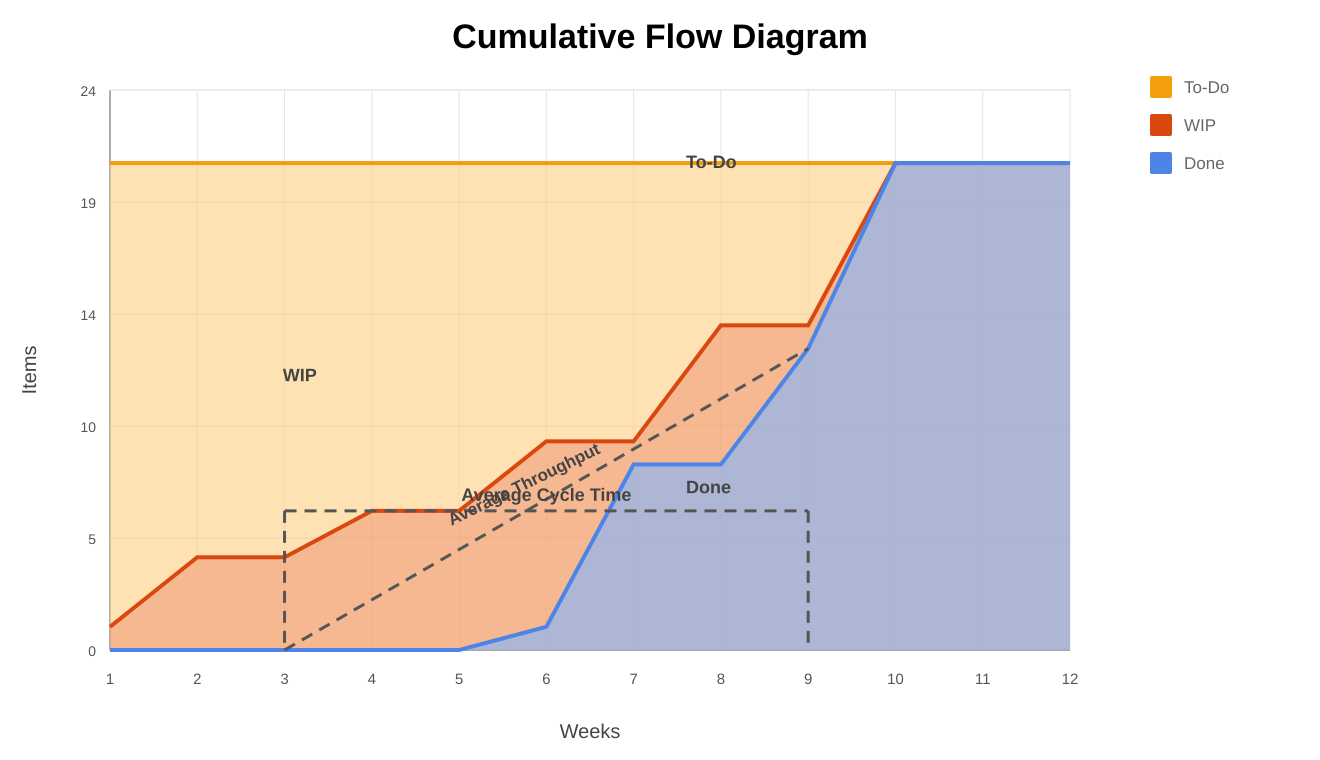
\includegraphics[width=0.92\linewidth]{figures/cfd.png}
\end{center}

The connected story here is that work did not close uniformly. The CFD shows that a significant amount of scope remained in progress until later sprints, which means the team was relying on staged maturity: foundation first, workflow next, operational modules after that, and only then full integration. That makes sense for this project, but it also explains why Sprint 5 felt dense.

\subsection{Throughput Report}
Throughput was measured at two levels: completed work items by sprint and feature-delivery behavior by git history. The first view shows sprint-level closure, while the second view shows the weekly bursts in which feature completions were actually recorded.

\begin{center}
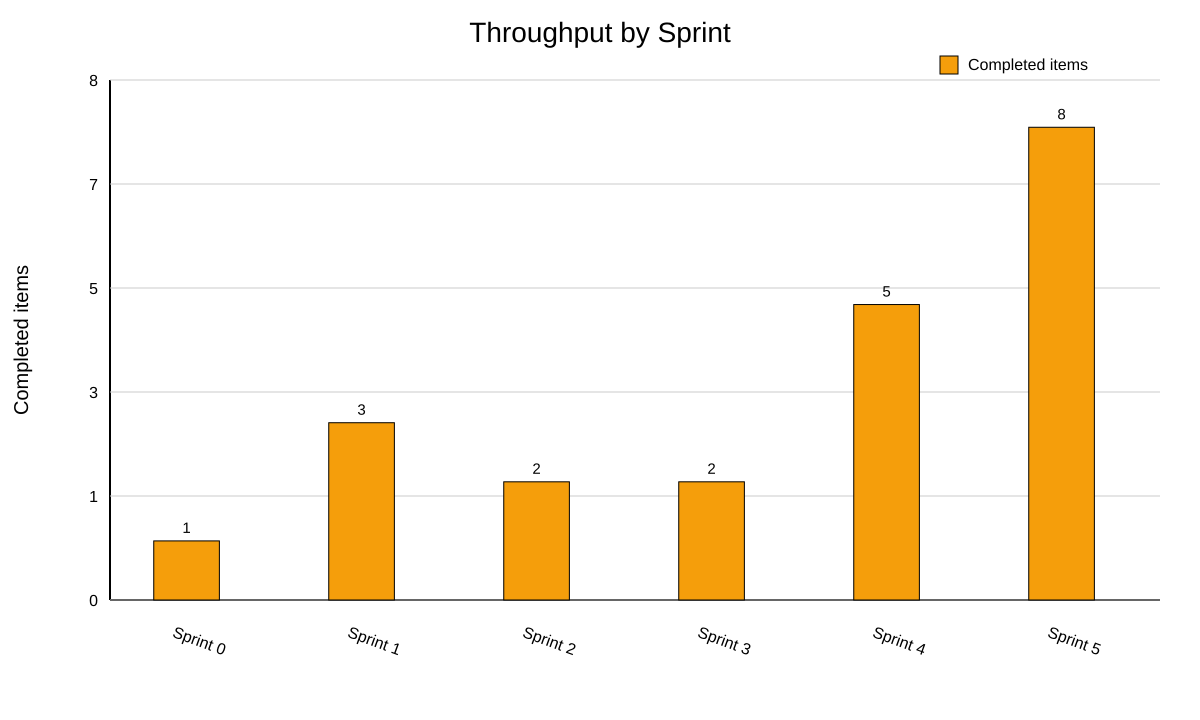
\includegraphics[width=0.92\linewidth]{figures/throughput.png}
\end{center}

\begin{center}
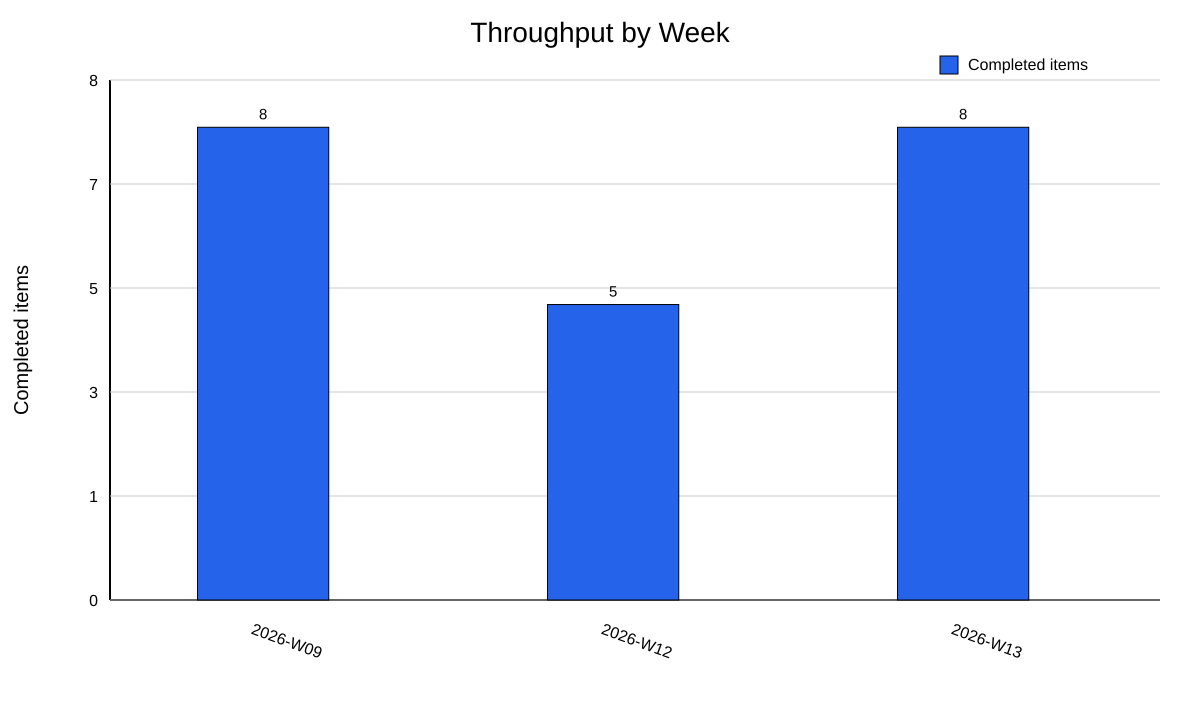
\includegraphics[width=0.92\linewidth]{figures/throughput_week.png}
\end{center}

The important observation is that throughput increases toward Sprint 4 and Sprint 5 instead of being flat across the semester. The weekly view shows that this closure did not happen smoothly; it happened in concentrated bursts, which is consistent with the late-sprint convergence already visible in the burn and cumulative-flow story. That is a real signal, not noise. It tells us that once the backend architecture stabilized, the team accelerated feature closure, but at the cost of a more compressed integration phase.

\subsection{Project Burndown and Burnup}
Because the prompt explicitly allows telling the test and project story in our own way, we chose project-wide burn charts instead of a narrow single-sprint chart. This gives a more honest picture of how scope accumulated and how completion caught up over time.

\begin{center}
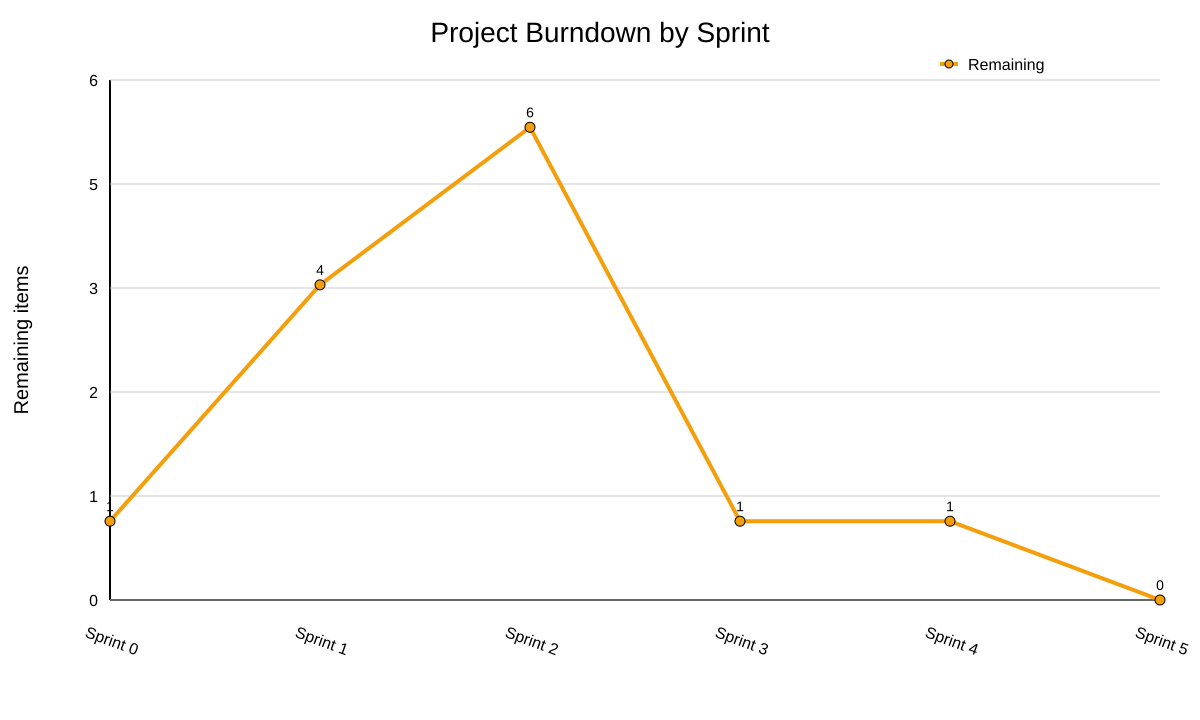
\includegraphics[width=0.92\linewidth]{figures/burndown.png}
\end{center}

\begin{center}
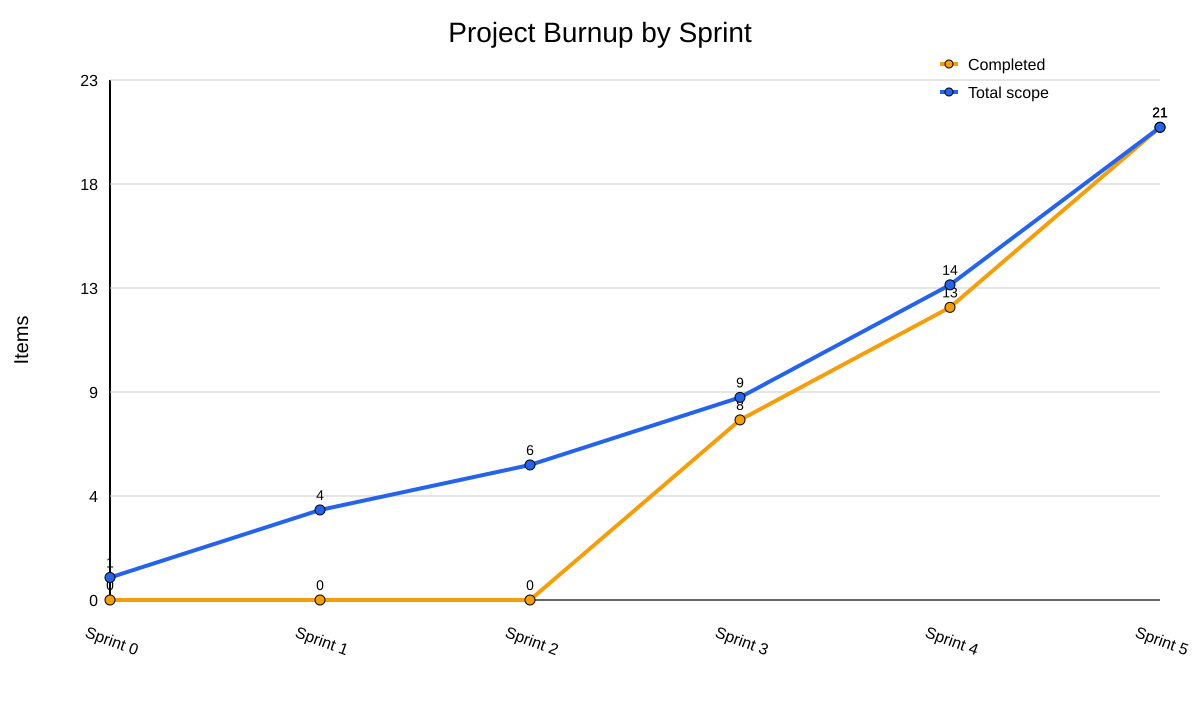
\includegraphics[width=0.92\linewidth]{figures/burnup.png}
\end{center}

The burndown and burnup together tell a coherent story. Scope expanded in a planned way from Sprint 0 through Sprint 5, but completion rose in steps rather than smoothly. That means the main process weakness was not uncontrolled scope growth; it was late visible closure. This distinction matters because the mitigation is not to reduce ambition, but to make integration and documentation visible earlier.

\subsection{Additional Metric 1: Team Velocity}
Team velocity was measured as completed work items per sprint. Unlike the throughput section, which emphasizes delivery timing at both sprint and weekly levels, this chart emphasizes the team's sustained closure capacity from sprint to sprint.

\begin{center}
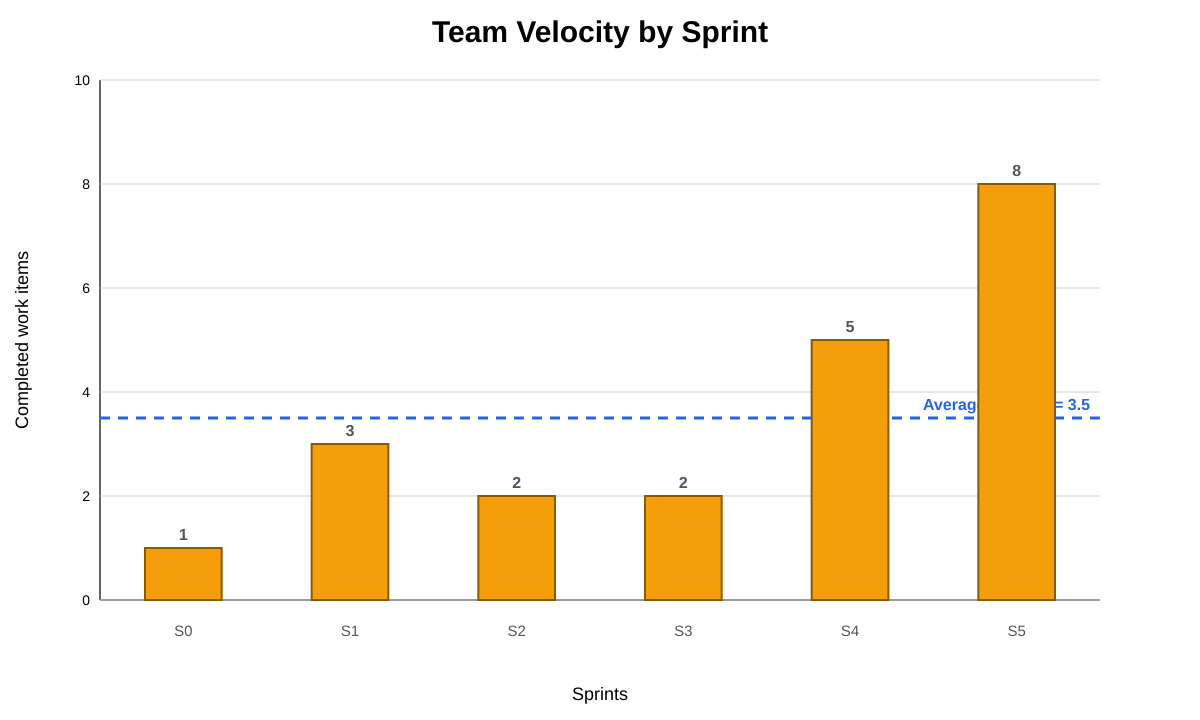
\includegraphics[width=0.92\linewidth]{figures/velocity.png}
\end{center}

The velocity story is consistent with the rest of the report: early sprints built the foundation, middle sprints established clinical workflows, and the strongest closure rate appeared in Sprint 4 and Sprint 5 once the architecture stabilized and the team could complete larger integrated slices. This makes the backend-first delivery pattern easy to see without reducing the story to raw commit counts.

\subsection{Additional Metric 2: Test and Performance Story}
The second additional metric is a combined quality story: pass rate and NFR timing compliance. The repository currently documents 48 categorized test cases in the CSV, all marked PASS, while the broader smoke automation has grown to 59 checks.

\begin{center}
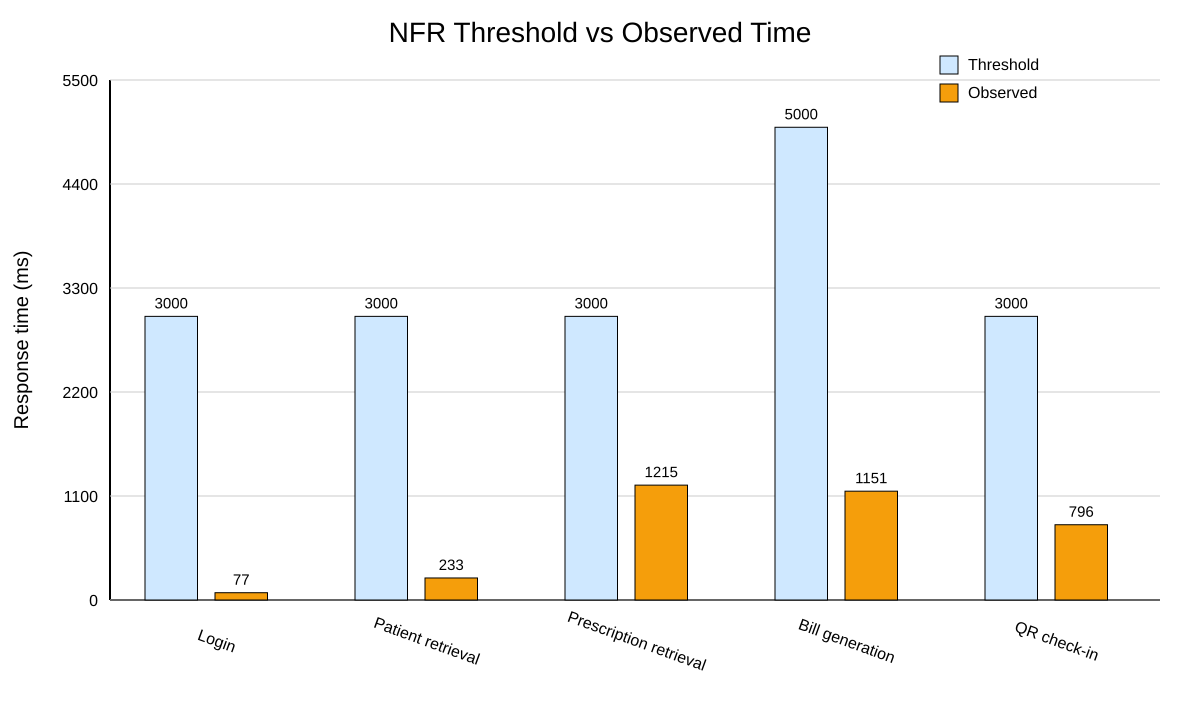
\includegraphics[width=0.92\linewidth]{figures/nfr.png}
\end{center}

The chart shows that all observed timings remain comfortably inside the stated thresholds. Login, patient retrieval, prescription retrieval, bill generation, and QR check-in all stay within the bounds defined in the project’s testing narrative. The positive result is that functional maturity and performance sanity were achieved together. The caution is that documentation synchronization became a project risk once the smoke suite grew beyond the 48-case CSV.

\section{Section II: Risk Analysis}
\subsection{Why a 5x5 Matrix Fits This Project}
The attached template suggests a classic 5x5 probability-impact matrix. That is appropriate here because the PHC system is not dominated by one catastrophic technical unknown; instead, it faces multiple moderate-to-high operational and integration risks that need prioritization. We therefore use the following scale. \textbf{Probability:} 1 = Rare, 2 = Unlikely, 3 = Moderate, 4 = Likely, 5 = Almost Certain. \textbf{Impact:} 1 = Insignificant, 2 = Minor, 3 = Significant, 4 = Major, 5 = Severe. \textbf{Risk score:} \(Probability \times Impact\).

\subsection{5x5 Risk Matrix}
\begin{center}
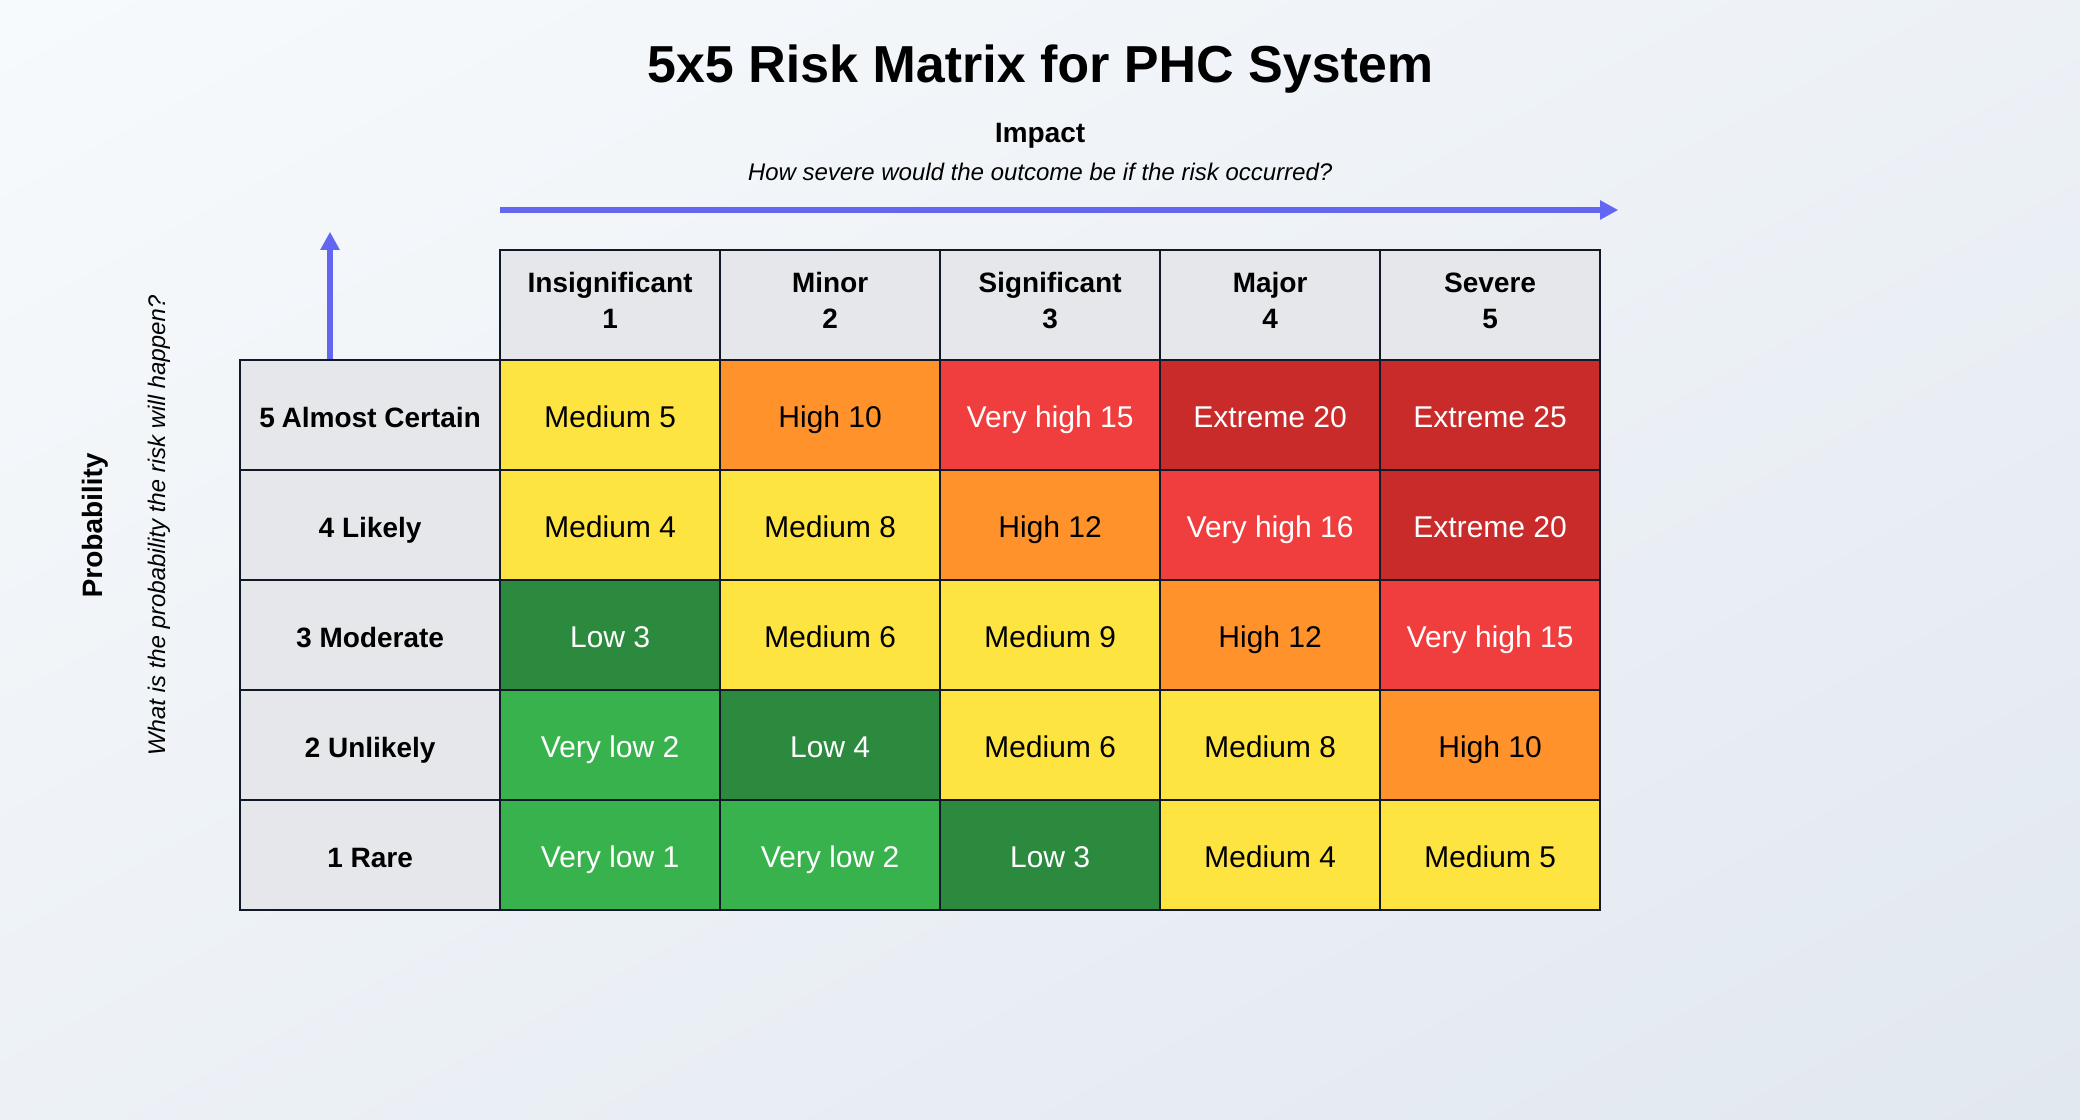
\includegraphics[width=0.98\linewidth]{figures/risk_matrix.png}
\end{center}

\subsection{Project-Specific Risk Register}
The matrix above provides the visual prioritization frame. For the formal project risk register, we map the PHC system onto the 14 standard risk classes from the provided template and evaluate them using project evidence from the SRS revisions, sprint logs, backend integration work, testing history, and the current state of frontend readiness. The assumed probabilities are based on a combination of repository evidence and team experience: risks already observed in some form during development, such as documentation drift, late-sprint convergence, integration pressure, or environment setup friction, are assigned higher probabilities; risks that remain plausible but were only weakly observed are kept in the low-to-medium range. \textbf{Impact codes:} C = Critical, S = Serious, Mo = Moderate, Mi = Minor.

\begin{center}
\rowcolors{2}{SoftGray}{white}
\begin{longtable}{|p{0.8cm}|p{4.9cm}|p{2.1cm}|p{1.4cm}|p{1.9cm}|}
\hline
\rowcolor{SoftBlue}
\textbf{ID} & \textbf{Risk} & \textbf{Probability (\%)} & \textbf{Impact} & \textbf{Level} \\
\hline
1 & Mission and Goals & 15 & C & Medium \\
\hline
2 & Program Management & 35 & S & Medium \\
\hline
3 & Decision Drivers & 20 & Mo & Low \\
\hline
4 & Organization Management & 25 & Mo & Low \\
\hline
5 & Customer/User & 45 & S & High \\
\hline
6 & Project Parameters & 40 & Mo & Medium \\
\hline
7 & Product Content & 55 & C & High \\
\hline
8 & Deployment & 30 & S & Medium \\
\hline
9 & Development Process & 50 & Mo & Medium \\
\hline
10 & Development Environment & 35 & Mi & Low \\
\hline
11 & Project Management & 60 & S & High \\
\hline
12 & Project Team & 45 & Mo & Medium \\
\hline
13 & Technology & 30 & Mo & Medium \\
\hline
14 & Maintenance & 20 & Mi & Low \\
\hline
\end{longtable}
\end{center}

These values are project-specific rather than generic. For example, \emph{Product Content} is high because the system now spans visits, prescriptions, lab workflows, billing, documents, notifications, reports, and access control; \emph{Customer/User} is high because the backend is mature while the end-user interface is still pending; and \emph{Project Management} is high because visible closure was concentrated in late sprints, increasing schedule sensitivity near the milestone. In other words, the probability estimates are not arbitrary numbers; they are reasoned estimates derived from our observed development pattern and from practical software-project judgment about which risks tend to recur once similar signals appear.

\section{Section III: Mapping Risk Mitigation to Sprint Planning}
This final section is where the report becomes a connected story instead of a list of charts. The project did not merely \emph{have} risks; it already responded to them through sprint ordering.

\begin{center}
\rowcolors{2}{SoftGray}{white}
\begin{tabular}{|p{1.3cm}|p{4cm}|p{7.7cm}|}
\hline
\rowcolor{SoftBlue}
\textbf{Sprint} & \textbf{Main risks addressed} & \textbf{How mitigation entered the backlog} \\
\hline
Sprint 0 & Scope ambiguity & Initial SRS revisions and UML work narrowed the project away from ambulance-style scope and toward a PHC-centered system. \\
\hline
Sprint 1 & Auth, storage, and requirement instability & Authentication, schema, and patient profile work were pulled first so all later modules had a stable identity and persistence base. \\
\hline
Sprint 2 & Workflow inconsistency & The team implemented visit lifecycle and doctor availability before prescriptions or labs, reducing downstream rework risk. \\
\hline
Sprint 3 & Clinical-module fragmentation & Prescriptions and lab requests were added only after consultation and queueing existed, which kept clinical flows coherent. \\
\hline
Sprint 4 & Transaction and operational risk & Billing and check-in were implemented with transaction-safe design, and operational modules were integrated without changing the visit-centric backbone. \\
\hline
Sprint 5 & Integration, documentation, auth hardening & Admin modules, notifications, E2E flow validation, API documentation, and real local LDAP support were explicitly added as mitigation work, not just as features. \\
\hline
Sprint 6 & Backend/UI imbalance & The current plan is to convert the stable API into role dashboards rather than reopen backend scope. \\
\hline
Sprint 7 & Release-readiness risk & Testing depth, RBAC verification, security hardening, load checks, and deployment preparation are reserved for the stabilization sprint. \\
\hline
\end{tabular}
\end{center}

This is the clearest way to tell the project story: the sprint order itself is a risk-mitigation strategy. The team did not just build modules in arbitrary order. It used ordering to reduce structural risk first, workflow risk next, operational risk later, and integration risk near backend closeout.

\section{Conclusion}
The PHC Integrated Digital System now has a strong backend story backed by measurable evidence. The COCOMO estimate places it in a meaningful engineering range, the Halstead and function-point results show non-trivial complexity, the flow and throughput charts show how work matured over time, and the test/performance data shows that the backend is not only large enough to matter but also stable enough to demonstrate.

The deeper conclusion, however, is about project control. The team’s real challenge is no longer \emph{whether} it can build the backend. It already has. The real challenge is how to convert that backend maturity into a coherent final product by keeping documentation aligned, making Sprint 6 visible, and using Sprint 7 for hardening instead of feature creep. That is why this report tells one connected story: metrics, risks, and sprint planning are not separate topics in this project. They are three views of the same development reality.

\section*{Progress Tracker}
\href{https://docs.google.com/spreadsheets/d/1xLa2L8eWv8gfrIwPXrnImF8uManlRlRwRp3ksSOVI9E/edit?usp=sharing}{Project tracker spreadsheet}

\end{document}
